
\chapter{Statistiques à deux variables quantitatives}
\competences{représenter, choisir un ajustement, interpoler, extrapoler avec prudence, communiquer}
\section{Cours de référence}
Une série statistique à deux variables est constituée de couples $(x_i,y_i)$. Le nuage de points permet d'observer une tendance, une dispersion et d'éventuelles valeurs atypiques.

\begin{center}
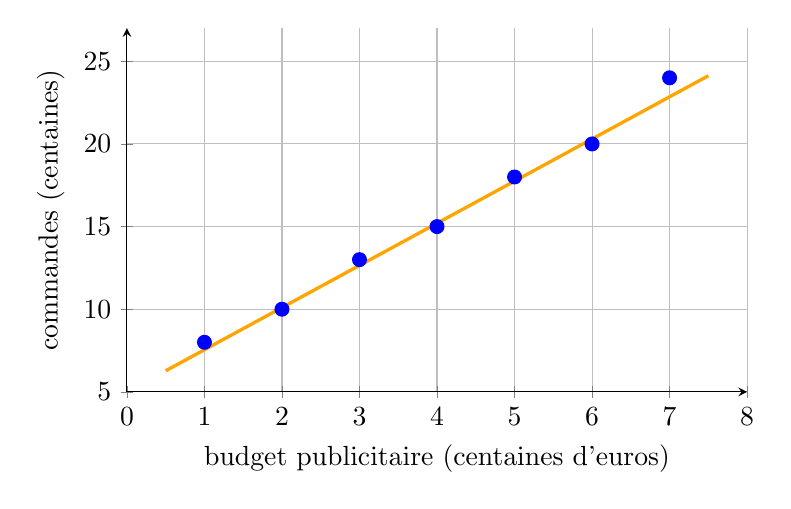
\begin{tikzpicture}
\begin{axis}[width=.78\textwidth,height=6.2cm,axis lines=left,xmin=0,xmax=8,ymin=5,ymax=27,grid=major,xlabel={budget publicitaire (centaines d'euros)},ylabel={commandes (centaines)}]
\addplot[only marks,mark=*,Blue,mark size=2.5pt] coordinates {(1,8)(2,10)(3,13)(4,15)(5,18)(6,20)(7,24)};
\addplot[Orange,very thick,domain=.5:7.5]{2.55*x+5};
\end{axis}
\end{tikzpicture}
\end{center}

\begin{retenir}
Une droite d'ajustement $y=ax+b$ fournit des estimations, pas des égalités exactes. Le coefficient $a$ décrit la variation moyenne estimée de $y$ quand $x$ augmente d'une unité. Une interpolation reste dans l'intervalle des valeurs observées ; une extrapolation sort de cet intervalle et doit être présentée avec prudence.
\end{retenir}

Le point moyen $G(\bar x,\bar y)$ a pour coordonnées $\bar x=\dfrac{x_1+\cdots+x_n}{n}$ et $\bar y=\dfrac{y_1+\cdots+y_n}{n}$. Une droite de régression obtenue à la calculatrice passe par $G$, à l'arrondi près.

\begin{methode}
Pour exploiter $y=ax+b$ : 1) remplacer $x$ par la valeur demandée pour estimer $y$ ; 2) résoudre $ax+b=y_0$ pour estimer $x$ ; 3) arrondir selon le contexte ; 4) préciser interpolation ou extrapolation ; 5) rappeler que le résultat dépend du modèle.
\end{methode}

Un changement de variable, par exemple $z=\log(y)$ ou $z=\dfrac1y$, peut rendre un nuage approximativement aligné. On ajuste alors $(x,z)$, puis on revient à la variable $y$.

\sessionheader{31}{26/01/2027}{B : 2 h -- C : 1 h}{Nuage de points}{Statistiques à deux variables}
\begin{objectifs}\begin{itemize}\item Construire un nuage.\item Choisir les échelles.\item Identifier les variables.\end{itemize}\end{objectifs}
\begin{automatismes}\begin{enumerate}\item Écrire le coefficient multiplicateur d'une hausse de $10\,\%$. \rep{$1+\dfrac{10}{100}=1,10$}\item Résoudre $3x+4=25$. \rep{$x=7$}\item Calculer la moyenne de $6$, $8$ et $10$. \rep{$8$}\item Donner la pente entre $(1,3)$ et $(4,9)$. \rep{$\dfrac{9-3}{4-1}=2$}\item Avec $y=2x+5$, calculer $y$ pour $x=7$. \rep{$19$}\end{enumerate}\end{automatismes}
\begin{prerequis}Relire la dernière trace écrite et savoir effectuer les calculs élémentaires mobilisés aujourd'hui. Avant l'activité, faire reformuler les mots-clés : construire un nuage et choisir les échelles.\end{prerequis}

\begin{activite}
Le tableau $(x_i,y_i)$ donne les dépenses publicitaires et les ventes de six mois : $(1,12),(2,15),(3,17),(4,22),(5,24),(6,28)$. Choisir des échelles, tracer le nuage et placer le point moyen.
\begin{center}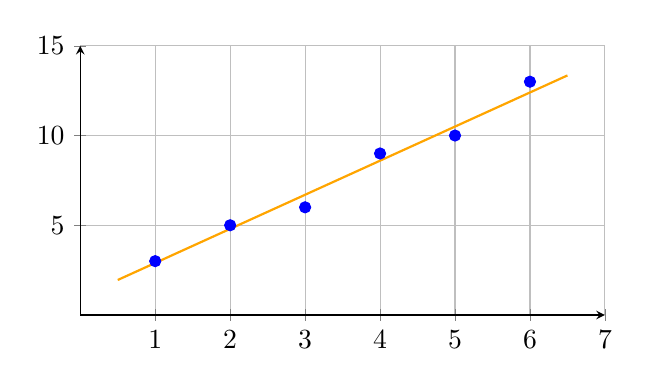
\begin{tikzpicture}\begin{axis}[width=.68\textwidth,height=5cm,axis lines=middle,xmin=0,xmax=7,ymin=0,ymax=15,grid=major]\addplot[only marks,Blue,mark=*] coordinates {(1,3)(2,5)(3,6)(4,9)(5,10)(6,13)};\addplot[Orange,thick,domain=.5:6.5]{1.9*x+1};\end{axis}\end{tikzpicture}\end{center}
\end{activite}
\enseignant{$\bar x=3{,}5$ et $\bar y=19{,}67$ environ. Le nuage présente une tendance croissante approximativement affine. Faire verbaliser la donnée qui déclenche le choix de méthode.}

\begin{traceecrite}Un nuage de points représente les couples $(x_i,y_i)$. Les axes, unités et échelles doivent être indiqués ; chaque couple donne un seul point.\end{traceecrite}

\begin{exemple}
Reprendre les données de l'activité et rédiger la solution dans l'ordre : définition des objets, propriété utilisée, calcul exact ou approché, puis phrase de réponse. La réponse modèle figure dans l'édition enseignant.
\end{exemple}
\enseignant{$\bar x=3{,}5$ et $\bar y=19{,}67$ environ. Le nuage présente une tendance croissante approximativement affine.}

\begin{exercice}[-- essentiel]
\begin{enumerate}\item Pour $y=3x+13$, estimer $y$ lorsque $x=8$.\item Résoudre $3x+13=50$.\item Le modèle a été établi sur $[2,12]$ : qualifier les estimations pour $x=8$ et $x=30$.\end{enumerate}
\end{exercice}
\enseignant{Pour $x=8$, $y=37$. L'équation donne $x=\dfrac{37}{3}$. $x=8$ donne une interpolation ; $x=30$ une extrapolation.}

\manuelref{Calao, cours p. 110--113 ; exercices p. 114, n° 1 à 6}
\CalaoSession{31}

\begin{dm}Reprendre l'exercice d'entraînement 2 avec les données suivantes : remplacer la donnée initiale par $275$ et le taux ou la raison par $3$. Rédiger en quatre lignes : données, formule, calcul, conclusion.\end{dm}
\enseignant{La correction dépend de l'exercice repris. Vérifier surtout la cohérence du modèle, le nombre d'itérations, l'arrondi et la phrase de conclusion.}

\begin{sortie}Sur une demi-feuille : écrire la règle principale de la séance, traiter un exemple très court et indiquer son degré de confiance de 1 à 4. Question(s) essentielle(s) du jour : 1, 2 et 3.\end{sortie}

\ifprof
\begin{methode}
\textbf{Conduite en 1 h :} 7 min d'automatismes ; 10 min de mise en commun et trace ; 28 min d'exercices essentiels ; 5 min de correction ; 3 min de billet de sortie.\\
\textbf{Conduite en 2 h :} ajouter 20 min de recherche de l'activité, 20 min d'institutionnalisation, un second exercice autonome et 10 min de correction comparée.\\
\textbf{Différenciation :} fournir aux élèves fragiles une fiche à quatre cases (données, modèle, calcul, conclusion). Demander aux élèves rapides de produire un contre-exemple, une justification ou une seconde méthode.
\end{methode}
\fi
\sessionheader{32}{28/01/2027}{B : 1 h -- C : 2 h}{Lecture et interprétation du nuage}{Statistiques à deux variables}
\begin{objectifs}\begin{itemize}\item Décrire une tendance.\item Repérer dispersion et atypiques.\item Éviter causalité abusive.\end{itemize}\end{objectifs}
\begin{automatismes}\begin{enumerate}\item Réduire $3x+7-x+2$. \rep{$2x+9$}\item Calculer la moyenne de $7$, $9$ et $11$. \rep{$9$}\item Donner la pente entre $(1,3)$ et $(4,9)$. \rep{$\dfrac{9-3}{4-1}=2$}\item Avec $y=2x+5$, calculer $y$ pour $x=7$. \rep{$19$}\item Résoudre $3x+4=25$. \rep{$x=7$}\end{enumerate}\end{automatismes}
\begin{prerequis}Relire la dernière trace écrite et savoir effectuer les calculs élémentaires mobilisés aujourd'hui. Avant l'activité, faire reformuler les mots-clés : décrire une tendance et repérer dispersion et atypiques.\end{prerequis}

\begin{activite}
Comparer trois nuages : tendance croissante serrée, tendance décroissante dispersée, absence de tendance. Rédiger pour chacun deux phrases sans employer le mot « cause ».

\end{activite}
\enseignant{La description porte sur direction, forme, dispersion et atypiques. Un nuage ne permet pas à lui seul d'établir une causalité. Faire verbaliser la donnée qui déclenche le choix de méthode.}

\begin{traceecrite}Décrire un nuage consiste à commenter la direction, la forme, la dispersion et les valeurs atypiques, sans affirmer une causalité non établie.\end{traceecrite}

\begin{exemple}
Reprendre les données de l'activité et rédiger la solution dans l'ordre : définition des objets, propriété utilisée, calcul exact ou approché, puis phrase de réponse. La réponse modèle figure dans l'édition enseignant.
\end{exemple}
\enseignant{La description porte sur direction, forme, dispersion et atypiques. Un nuage ne permet pas à lui seul d'établir une causalité.}

\begin{exercice}[-- essentiel]
\begin{enumerate}\item Pour $y=4x+14$, estimer $y$ lorsque $x=8$.\item Résoudre $4x+14=50$.\item Le modèle a été établi sur $[2,12]$ : qualifier les estimations pour $x=8$ et $x=30$.\end{enumerate}
\end{exercice}
\enseignant{Pour $x=8$, $y=46$. L'équation donne $x=\dfrac{36}{4}$. $x=8$ donne une interpolation ; $x=30$ une extrapolation.}

\manuelref{Calao, p. 116, n° 11 à 15}
\CalaoSession{32}

\begin{dm}Reprendre l'exercice d'entraînement 3 avec les données suivantes : remplacer la donnée initiale par $280$ et le taux ou la raison par $4$. Rédiger en quatre lignes : données, formule, calcul, conclusion.\end{dm}
\enseignant{La correction dépend de l'exercice repris. Vérifier surtout la cohérence du modèle, le nombre d'itérations, l'arrondi et la phrase de conclusion.}

\begin{sortie}Sur une demi-feuille : écrire la règle principale de la séance, traiter un exemple très court et indiquer son degré de confiance de 1 à 4. Question(s) essentielle(s) du jour : 1 et 2.\end{sortie}

\ifprof
\begin{methode}
\textbf{Conduite en 1 h :} 7 min d'automatismes ; 10 min de mise en commun et trace ; 28 min d'exercices essentiels ; 5 min de correction ; 3 min de billet de sortie.\\
\textbf{Conduite en 2 h :} ajouter 20 min de recherche de l'activité, 20 min d'institutionnalisation, un second exercice autonome et 10 min de correction comparée.\\
\textbf{Différenciation :} fournir aux élèves fragiles une fiche à quatre cases (données, modèle, calcul, conclusion). Demander aux élèves rapides de produire un contre-exemple, une justification ou une seconde méthode.
\end{methode}
\fi
\sessionheader{33}{02/02/2027}{B : 2 h -- C : 1 h}{Ajustement affine}{Statistiques à deux variables}
\begin{objectifs}\begin{itemize}\item Obtenir un ajustement affine.\item Interpréter $a$ et $b$.\item Vérifier avec le point moyen.\end{itemize}\end{objectifs}
\begin{automatismes}\begin{enumerate}\item Calculer $20\,\%$ de $160$. \rep{$32$}\item Donner la pente entre $(1,3)$ et $(4,9)$. \rep{$\dfrac{9-3}{4-1}=2$}\item Avec $y=2x+5$, calculer $y$ pour $x=7$. \rep{$19$}\item Résoudre $3x+4=25$. \rep{$x=7$}\item Calculer la moyenne de $8$, $10$ et $12$. \rep{$10$}\end{enumerate}\end{automatismes}
\begin{prerequis}Relire la dernière trace écrite et savoir effectuer les calculs élémentaires mobilisés aujourd'hui. Avant l'activité, faire reformuler les mots-clés : obtenir un ajustement affine et interpréter $a$ et $b$.\end{prerequis}

\begin{activite}
Avec les données de la séance 31, obtenir la régression affine à la calculatrice. Interpréter la pente et vérifier que le point moyen appartient approximativement à la droite.
\begin{center}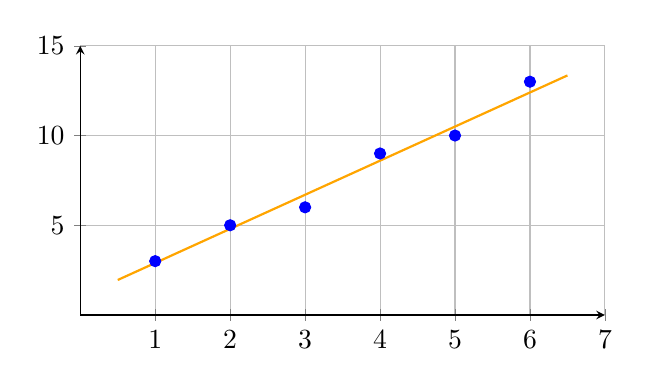
\begin{tikzpicture}\begin{axis}[width=.68\textwidth,height=5cm,axis lines=middle,xmin=0,xmax=7,ymin=0,ymax=15,grid=major]\addplot[only marks,Blue,mark=*] coordinates {(1,3)(2,5)(3,6)(4,9)(5,10)(6,13)};\addplot[Orange,thick,domain=.5:6.5]{1.9*x+1};\end{axis}\end{tikzpicture}\end{center}
\end{activite}
\enseignant{Une régression donne environ $y=3{,}17x+8{,}57$. Une centaine d'euros supplémentaire est associée à environ $317$ ventes supplémentaires si $y$ est en centaines. Faire verbaliser la donnée qui déclenche le choix de méthode.}

\begin{traceecrite}Une droite $y=ax+b$ ajuste un nuage. $a$ représente la variation moyenne estimée de $y$ pour une unité supplémentaire de $x$.\end{traceecrite}

\begin{exemple}
Reprendre les données de l'activité et rédiger la solution dans l'ordre : définition des objets, propriété utilisée, calcul exact ou approché, puis phrase de réponse. La réponse modèle figure dans l'édition enseignant.
\end{exemple}
\enseignant{Une régression donne environ $y=3{,}17x+8{,}57$. Une centaine d'euros supplémentaire est associée à environ $317$ ventes supplémentaires si $y$ est en centaines.}

\begin{exercice}[-- essentiel]
\begin{enumerate}\item Pour $y=5x+15$, estimer $y$ lorsque $x=8$.\item Résoudre $5x+15=50$.\item Le modèle a été établi sur $[2,12]$ : qualifier les estimations pour $x=8$ et $x=30$.\end{enumerate}
\end{exercice}
\enseignant{Pour $x=8$, $y=55$. L'équation donne $x=\dfrac{35}{5}$. $x=8$ donne une interpolation ; $x=30$ une extrapolation.}

\manuelref{Calao, cours p. 110--113 ; exercices p. 117, n° 16 à 18}
\CalaoSession{33}

\begin{dm}Reprendre l'exercice d'entraînement 2 avec les données suivantes : remplacer la donnée initiale par $285$ et le taux ou la raison par $5$. Rédiger en quatre lignes : données, formule, calcul, conclusion.\end{dm}
\enseignant{La correction dépend de l'exercice repris. Vérifier surtout la cohérence du modèle, le nombre d'itérations, l'arrondi et la phrase de conclusion.}

\begin{sortie}Sur une demi-feuille : écrire la règle principale de la séance, traiter un exemple très court et indiquer son degré de confiance de 1 à 4. Question(s) essentielle(s) du jour : 1, 2 et 3.\end{sortie}

\ifprof
\begin{methode}
\textbf{Conduite en 1 h :} 7 min d'automatismes ; 10 min de mise en commun et trace ; 28 min d'exercices essentiels ; 5 min de correction ; 3 min de billet de sortie.\\
\textbf{Conduite en 2 h :} ajouter 20 min de recherche de l'activité, 20 min d'institutionnalisation, un second exercice autonome et 10 min de correction comparée.\\
\textbf{Différenciation :} fournir aux élèves fragiles une fiche à quatre cases (données, modèle, calcul, conclusion). Demander aux élèves rapides de produire un contre-exemple, une justification ou une seconde méthode.
\end{methode}
\fi
\sessionheader{34}{04/02/2027}{B : 1 h -- C : 2 h}{Interpolation}{Statistiques à deux variables}
\begin{objectifs}\begin{itemize}\item Interpoler.\item Résoudre avec le modèle.\item Exprimer une estimation.\end{itemize}\end{objectifs}
\begin{automatismes}\begin{enumerate}\item Écrire le coefficient multiplicateur d'une hausse de $25\,\%$. \rep{$1+\dfrac{25}{100}=1,25$}\item Avec $y=2x+5$, calculer $y$ pour $x=7$. \rep{$19$}\item Résoudre $3x+4=25$. \rep{$x=7$}\item Calculer la moyenne de $9$, $11$ et $13$. \rep{$11$}\item Donner la pente entre $(1,3)$ et $(4,9)$. \rep{$\dfrac{9-3}{4-1}=2$}\end{enumerate}\end{automatismes}
\begin{prerequis}Relire la dernière trace écrite et savoir effectuer les calculs élémentaires mobilisés aujourd'hui. Avant l'activité, faire reformuler les mots-clés : interpoler et résoudre avec le modèle.\end{prerequis}

\begin{activite}
Sur la période observée $x\in[1,12]$, le modèle est $y=2{,}8x+14$. Estimer $y$ pour $x=7{,}5$, puis estimer $x$ lorsque $y=35$. Qualifier chaque estimation.
\begin{center}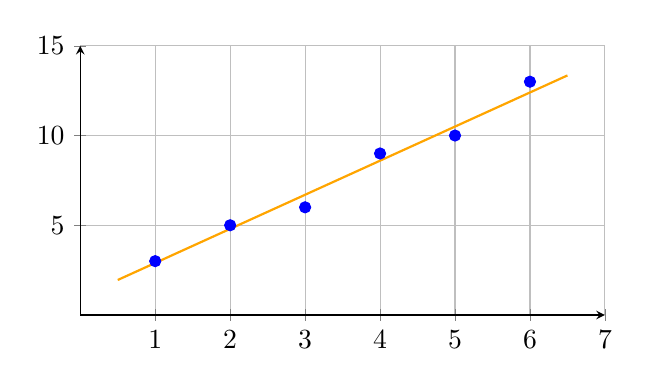
\begin{tikzpicture}\begin{axis}[width=.68\textwidth,height=5cm,axis lines=middle,xmin=0,xmax=7,ymin=0,ymax=15,grid=major]\addplot[only marks,Blue,mark=*] coordinates {(1,3)(2,5)(3,6)(4,9)(5,10)(6,13)};\addplot[Orange,thick,domain=.5:6.5]{1.9*x+1};\end{axis}\end{tikzpicture}\end{center}
\end{activite}
\enseignant{$y=35$ et $x=7{,}5$. Les deux valeurs sont à l'intérieur de l'intervalle observé : interpolations. Faire verbaliser la donnée qui déclenche le choix de méthode.}

\begin{traceecrite}Une interpolation estime une valeur à l'intérieur de l'intervalle observé. Le résultat est une estimation dépendante du modèle.\end{traceecrite}

\begin{exemple}
Reprendre les données de l'activité et rédiger la solution dans l'ordre : définition des objets, propriété utilisée, calcul exact ou approché, puis phrase de réponse. La réponse modèle figure dans l'édition enseignant.
\end{exemple}
\enseignant{$y=35$ et $x=7{,}5$. Les deux valeurs sont à l'intérieur de l'intervalle observé : interpolations.}

\begin{exercice}[-- essentiel]
\begin{enumerate}\item Pour $y=6x+16$, estimer $y$ lorsque $x=8$.\item Résoudre $6x+16=50$.\item Le modèle a été établi sur $[2,12]$ : qualifier les estimations pour $x=8$ et $x=30$.\end{enumerate}
\end{exercice}
\enseignant{Pour $x=8$, $y=64$. L'équation donne $x=\dfrac{34}{6}$. $x=8$ donne une interpolation ; $x=30$ une extrapolation.}

\manuelref{Calao, p. 118, n° 19 à 24}
\CalaoSession{34}

\begin{dm}Reprendre l'exercice d'entraînement 3 avec les données suivantes : remplacer la donnée initiale par $290$ et le taux ou la raison par $6$. Rédiger en quatre lignes : données, formule, calcul, conclusion.\end{dm}
\enseignant{La correction dépend de l'exercice repris. Vérifier surtout la cohérence du modèle, le nombre d'itérations, l'arrondi et la phrase de conclusion.}

\begin{sortie}Sur une demi-feuille : écrire la règle principale de la séance, traiter un exemple très court et indiquer son degré de confiance de 1 à 4. Question(s) essentielle(s) du jour : 1 et 2.\end{sortie}

\ifprof
\begin{methode}
\textbf{Conduite en 1 h :} 7 min d'automatismes ; 10 min de mise en commun et trace ; 28 min d'exercices essentiels ; 5 min de correction ; 3 min de billet de sortie.\\
\textbf{Conduite en 2 h :} ajouter 20 min de recherche de l'activité, 20 min d'institutionnalisation, un second exercice autonome et 10 min de correction comparée.\\
\textbf{Différenciation :} fournir aux élèves fragiles une fiche à quatre cases (données, modèle, calcul, conclusion). Demander aux élèves rapides de produire un contre-exemple, une justification ou une seconde méthode.
\end{methode}
\fi
\sessionheader{35}{09/02/2027}{B : 2 h -- C : 1 h}{Extrapolation}{Statistiques à deux variables}
\begin{objectifs}\begin{itemize}\item Extrapoler prudemment.\item Évaluer la plausibilité.\item Présenter une limite du modèle.\end{itemize}\end{objectifs}
\begin{automatismes}\begin{enumerate}\item Réduire $3x+3-x+2$. \rep{$2x+5$}\item Résoudre $3x+4=25$. \rep{$x=7$}\item Calculer la moyenne de $3$, $5$ et $7$. \rep{$5$}\item Donner la pente entre $(1,3)$ et $(4,9)$. \rep{$\dfrac{9-3}{4-1}=2$}\item Avec $y=2x+5$, calculer $y$ pour $x=7$. \rep{$19$}\end{enumerate}\end{automatismes}
\begin{prerequis}Relire la dernière trace écrite et savoir effectuer les calculs élémentaires mobilisés aujourd'hui. Avant l'activité, faire reformuler les mots-clés : extrapoler prudemment et évaluer la plausibilité.\end{prerequis}

\begin{activite}
Le même modèle $y=2{,}8x+14$, ajusté sur $[1,12]$, est utilisé pour $x=40$. Calculer l'estimation, puis donner trois raisons pour lesquelles elle peut être peu fiable.
\begin{center}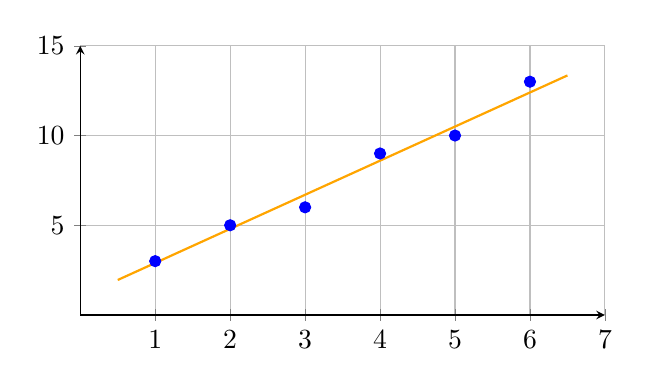
\begin{tikzpicture}\begin{axis}[width=.68\textwidth,height=5cm,axis lines=middle,xmin=0,xmax=7,ymin=0,ymax=15,grid=major]\addplot[only marks,Blue,mark=*] coordinates {(1,3)(2,5)(3,6)(4,9)(5,10)(6,13)};\addplot[Orange,thick,domain=.5:6.5]{1.9*x+1};\end{axis}\end{tikzpicture}\end{center}
\end{activite}
\enseignant{L'estimation vaut $126$. Elle est éloignée des données, la tendance peut changer et des contraintes réelles peuvent plafonner la variable. Faire verbaliser la donnée qui déclenche le choix de méthode.}

\begin{traceecrite}Une extrapolation estime hors de l'intervalle observé. Plus on s'en éloigne, plus la prudence est nécessaire.\end{traceecrite}

\begin{exemple}
Reprendre les données de l'activité et rédiger la solution dans l'ordre : définition des objets, propriété utilisée, calcul exact ou approché, puis phrase de réponse. La réponse modèle figure dans l'édition enseignant.
\end{exemple}
\enseignant{L'estimation vaut $126$. Elle est éloignée des données, la tendance peut changer et des contraintes réelles peuvent plafonner la variable.}

\begin{exercice}[-- essentiel]
\begin{enumerate}\item Pour $y=2x+12$, estimer $y$ lorsque $x=8$.\item Résoudre $2x+12=50$.\item Le modèle a été établi sur $[2,12]$ : qualifier les estimations pour $x=8$ et $x=30$.\end{enumerate}
\end{exercice}
\enseignant{Pour $x=8$, $y=28$. L'équation donne $x=\dfrac{38}{2}$. $x=8$ donne une interpolation ; $x=30$ une extrapolation.}

\manuelref{Calao, p. 119, n° 25 à 27}
\CalaoSession{35}

\begin{dm}Reprendre l'exercice d'entraînement 2 avec les données suivantes : remplacer la donnée initiale par $295$ et le taux ou la raison par $7$. Rédiger en quatre lignes : données, formule, calcul, conclusion.\end{dm}
\enseignant{La correction dépend de l'exercice repris. Vérifier surtout la cohérence du modèle, le nombre d'itérations, l'arrondi et la phrase de conclusion.}

\begin{sortie}Sur une demi-feuille : écrire la règle principale de la séance, traiter un exemple très court et indiquer son degré de confiance de 1 à 4. Question(s) essentielle(s) du jour : 1, 2 et 3.\end{sortie}

\ifprof
\begin{methode}
\textbf{Conduite en 1 h :} 7 min d'automatismes ; 10 min de mise en commun et trace ; 28 min d'exercices essentiels ; 5 min de correction ; 3 min de billet de sortie.\\
\textbf{Conduite en 2 h :} ajouter 20 min de recherche de l'activité, 20 min d'institutionnalisation, un second exercice autonome et 10 min de correction comparée.\\
\textbf{Différenciation :} fournir aux élèves fragiles une fiche à quatre cases (données, modèle, calcul, conclusion). Demander aux élèves rapides de produire un contre-exemple, une justification ou une seconde méthode.
\end{methode}
\fi
\sessionheader{36}{11/02/2027}{B : 1 h -- C : 2 h}{Changement de variable}{Statistiques à deux variables}
\begin{objectifs}\begin{itemize}\item Effectuer un changement de variable.\item Ajuster les nouvelles données.\item Revenir à la variable initiale.\end{itemize}\end{objectifs}
\begin{automatismes}\begin{enumerate}\item Calculer $5\,\%$ de $80$. \rep{$4$}\item Calculer la moyenne de $4$, $6$ et $8$. \rep{$6$}\item Donner la pente entre $(1,3)$ et $(4,9)$. \rep{$\dfrac{9-3}{4-1}=2$}\item Avec $y=2x+5$, calculer $y$ pour $x=7$. \rep{$19$}\item Résoudre $3x+4=25$. \rep{$x=7$}\end{enumerate}\end{automatismes}
\begin{prerequis}Relire la dernière trace écrite et savoir effectuer les calculs élémentaires mobilisés aujourd'hui. Avant l'activité, faire reformuler les mots-clés : effectuer un changement de variable et ajuster les nouvelles données.\end{prerequis}

\begin{activite}
Les données semblent exponentielles. On pose $z=\log(y)$ et l'ajustement donne $z=0{,}08x+1{,}2$. Exprimer $y$ en fonction de $x$, puis calculer $y$ pour $x=5$.

\end{activite}
\enseignant{$y=10^{0{,}08x+1{,}2}$. Pour $x=5$, $y=10^{1{,}6}\approx39{,}8$. Faire verbaliser la donnée qui déclenche le choix de méthode.}

\begin{traceecrite}Un changement de variable peut aligner un nuage. Après l'ajustement dans la nouvelle variable, il faut revenir à la variable initiale.\end{traceecrite}

\begin{exemple}
Reprendre les données de l'activité et rédiger la solution dans l'ordre : définition des objets, propriété utilisée, calcul exact ou approché, puis phrase de réponse. La réponse modèle figure dans l'édition enseignant.
\end{exemple}
\enseignant{$y=10^{0{,}08x+1{,}2}$. Pour $x=5$, $y=10^{1{,}6}\approx39{,}8$.}

\begin{exercice}[-- essentiel]
\begin{enumerate}\item Pour $y=3x+13$, estimer $y$ lorsque $x=8$.\item Résoudre $3x+13=50$.\item Le modèle a été établi sur $[2,12]$ : qualifier les estimations pour $x=8$ et $x=30$.\end{enumerate}
\end{exercice}
\enseignant{Pour $x=8$, $y=37$. L'équation donne $x=\dfrac{37}{3}$. $x=8$ donne une interpolation ; $x=30$ une extrapolation.}

\manuelref{Calao, p. 120, n° 28--29}
\CalaoSession{36}

\begin{dm}Reprendre l'exercice d'entraînement 3 avec les données suivantes : remplacer la donnée initiale par $300$ et le taux ou la raison par $2$. Rédiger en quatre lignes : données, formule, calcul, conclusion.\end{dm}
\enseignant{La correction dépend de l'exercice repris. Vérifier surtout la cohérence du modèle, le nombre d'itérations, l'arrondi et la phrase de conclusion.}

\begin{sortie}Sur une demi-feuille : écrire la règle principale de la séance, traiter un exemple très court et indiquer son degré de confiance de 1 à 4. Question(s) essentielle(s) du jour : 1 et 2.\end{sortie}

\ifprof
\begin{methode}
\textbf{Conduite en 1 h :} 7 min d'automatismes ; 10 min de mise en commun et trace ; 28 min d'exercices essentiels ; 5 min de correction ; 3 min de billet de sortie.\\
\textbf{Conduite en 2 h :} ajouter 20 min de recherche de l'activité, 20 min d'institutionnalisation, un second exercice autonome et 10 min de correction comparée.\\
\textbf{Différenciation :} fournir aux élèves fragiles une fiche à quatre cases (données, modèle, calcul, conclusion). Demander aux élèves rapides de produire un contre-exemple, une justification ou une seconde méthode.
\end{methode}
\fi
\sessionheader{37}{02/03/2027}{B : 2 h -- C : 1 h}{Choix du modèle et ajustement}{Statistiques à deux variables}
\begin{objectifs}\begin{itemize}\item Comparer des modèles.\item Utiliser les résidus.\item Définir un domaine d'usage.\end{itemize}\end{objectifs}
\begin{automatismes}\begin{enumerate}\item Écrire le coefficient multiplicateur d'une hausse de $10\,\%$. \rep{$1+\dfrac{10}{100}=1,10$}\item Donner la pente entre $(1,3)$ et $(4,9)$. \rep{$\dfrac{9-3}{4-1}=2$}\item Avec $y=2x+5$, calculer $y$ pour $x=7$. \rep{$19$}\item Résoudre $3x+4=25$. \rep{$x=7$}\item Calculer la moyenne de $5$, $7$ et $9$. \rep{$7$}\end{enumerate}\end{automatismes}
\begin{prerequis}Relire la dernière trace écrite et savoir effectuer les calculs élémentaires mobilisés aujourd'hui. Avant l'activité, faire reformuler les mots-clés : comparer des modèles et utiliser les résidus.\end{prerequis}

\begin{activite}
Deux modèles donnent des résidus absolus totaux $18{,}4$ et $11{,}7$ sur la zone observée. Le second comporte cependant une croissance irréaliste après $x=20$. Choisir un modèle pour interpoler à $x=12$, puis discuter l'extrapolation à $x=50$.
\begin{center}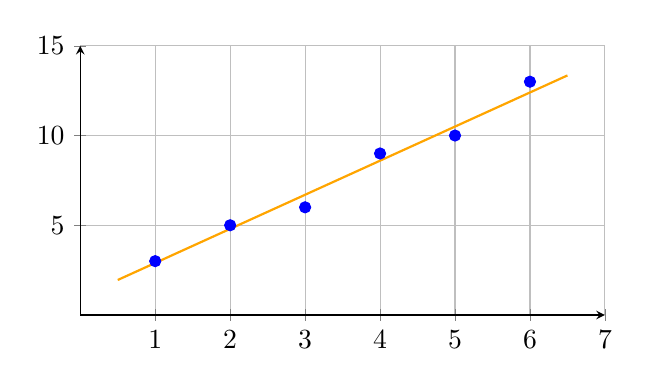
\begin{tikzpicture}\begin{axis}[width=.68\textwidth,height=5cm,axis lines=middle,xmin=0,xmax=7,ymin=0,ymax=15,grid=major]\addplot[only marks,Blue,mark=*] coordinates {(1,3)(2,5)(3,6)(4,9)(5,10)(6,13)};\addplot[Orange,thick,domain=.5:6.5]{1.9*x+1};\end{axis}\end{tikzpicture}\end{center}
\end{activite}
\enseignant{Le second est préférable pour interpoler sur la zone observée si les autres critères sont comparables ; aucun choix automatique n'est justifié pour $x=50$. Faire verbaliser la donnée qui déclenche le choix de méthode.}

\begin{traceecrite}On choisit un modèle selon la forme du nuage, la taille des résidus et le domaine d'usage. Un meilleur ajustement visuel n'autorise pas une extrapolation illimitée.\end{traceecrite}

\begin{exemple}
Reprendre les données de l'activité et rédiger la solution dans l'ordre : définition des objets, propriété utilisée, calcul exact ou approché, puis phrase de réponse. La réponse modèle figure dans l'édition enseignant.
\end{exemple}
\enseignant{Le second est préférable pour interpoler sur la zone observée si les autres critères sont comparables ; aucun choix automatique n'est justifié pour $x=50$.}

\begin{exercice}[-- essentiel]
\begin{enumerate}\item Pour $y=4x+14$, estimer $y$ lorsque $x=8$.\item Résoudre $4x+14=50$.\item Le modèle a été établi sur $[2,12]$ : qualifier les estimations pour $x=8$ et $x=30$.\end{enumerate}
\end{exercice}
\enseignant{Pour $x=8$, $y=46$. L'équation donne $x=\dfrac{36}{4}$. $x=8$ donne une interpolation ; $x=30$ une extrapolation.}

\manuelref{Calao, p. 121, n° 30 à 32, puis p. 122, n° 33}
\CalaoSession{37}

\begin{dm}Reprendre l'exercice d'entraînement 2 avec les données suivantes : remplacer la donnée initiale par $305$ et le taux ou la raison par $3$. Rédiger en quatre lignes : données, formule, calcul, conclusion.\end{dm}
\enseignant{La correction dépend de l'exercice repris. Vérifier surtout la cohérence du modèle, le nombre d'itérations, l'arrondi et la phrase de conclusion.}

\begin{sortie}Sur une demi-feuille : écrire la règle principale de la séance, traiter un exemple très court et indiquer son degré de confiance de 1 à 4. Question(s) essentielle(s) du jour : 1, 2 et 3.\end{sortie}

\ifprof
\begin{methode}
\textbf{Conduite en 1 h :} 7 min d'automatismes ; 10 min de mise en commun et trace ; 28 min d'exercices essentiels ; 5 min de correction ; 3 min de billet de sortie.\\
\textbf{Conduite en 2 h :} ajouter 20 min de recherche de l'activité, 20 min d'institutionnalisation, un second exercice autonome et 10 min de correction comparée.\\
\textbf{Différenciation :} fournir aux élèves fragiles une fiche à quatre cases (données, modèle, calcul, conclusion). Demander aux élèves rapides de produire un contre-exemple, une justification ou une seconde méthode.
\end{methode}
\fi
\sessionheader{38}{04/03/2027}{B : 1 h -- C : 2 h}{Bilan et évaluation}{Statistiques à deux variables}
\begin{objectifs}\begin{itemize}\item Choisir et exploiter un ajustement.\item Rédiger une conclusion statistique.\item Analyser une erreur.\end{itemize}\end{objectifs}
\begin{automatismes}\begin{enumerate}\item Réduire $3x+6-x+2$. \rep{$2x+8$}\item Avec $y=2x+5$, calculer $y$ pour $x=7$. \rep{$19$}\item Résoudre $3x+4=25$. \rep{$x=7$}\item Calculer la moyenne de $6$, $8$ et $10$. \rep{$8$}\item Donner la pente entre $(1,3)$ et $(4,9)$. \rep{$\dfrac{9-3}{4-1}=2$}\end{enumerate}\end{automatismes}
\begin{prerequis}Relire la dernière trace écrite et savoir effectuer les calculs élémentaires mobilisés aujourd'hui. Avant l'activité, faire reformuler les mots-clés : choisir et exploiter un ajustement et rédiger une conclusion statistique.\end{prerequis}

\begin{activite}
À partir d'un nuage fourni par le professeur, produire une réponse complète : choix du modèle, équation, estimation, type d'estimation, unité et réserve. Échanger les copies et utiliser une grille de six critères.

\end{activite}
\enseignant{La correction vérifie la cohérence du modèle et la présence des six éléments demandés, pas seulement le résultat numérique. Faire verbaliser la donnée qui déclenche le choix de méthode.}

\begin{traceecrite}Une réponse statistique complète contient le modèle, le calcul, l'arrondi, l'unité, le type d'estimation et une réserve sur la validité.\end{traceecrite}

\begin{exemple}
Reprendre les données de l'activité et rédiger la solution dans l'ordre : définition des objets, propriété utilisée, calcul exact ou approché, puis phrase de réponse. La réponse modèle figure dans l'édition enseignant.
\end{exemple}
\enseignant{La correction vérifie la cohérence du modèle et la présence des six éléments demandés, pas seulement le résultat numérique.}

\begin{exercice}[-- essentiel]
\begin{enumerate}\item Pour $y=5x+15$, estimer $y$ lorsque $x=8$.\item Résoudre $5x+15=50$.\item Le modèle a été établi sur $[2,12]$ : qualifier les estimations pour $x=8$ et $x=30$.\end{enumerate}
\end{exercice}
\enseignant{Pour $x=8$, $y=55$. L'équation donne $x=\dfrac{35}{5}$. $x=8$ donne une interpolation ; $x=30$ une extrapolation.}

\manuelref{Calao, p. 122--123}
\CalaoSession{38}

\begin{dm}Reprendre l'exercice d'entraînement 3 avec les données suivantes : remplacer la donnée initiale par $310$ et le taux ou la raison par $4$. Rédiger en quatre lignes : données, formule, calcul, conclusion.\end{dm}
\enseignant{La correction dépend de l'exercice repris. Vérifier surtout la cohérence du modèle, le nombre d'itérations, l'arrondi et la phrase de conclusion.}

\begin{sortie}Sur une demi-feuille : écrire la règle principale de la séance, traiter un exemple très court et indiquer son degré de confiance de 1 à 4. Question(s) essentielle(s) du jour : 1 et 2.\end{sortie}

\ifprof
\begin{methode}
\textbf{Conduite en 1 h :} 7 min d'automatismes ; 10 min de mise en commun et trace ; 28 min d'exercices essentiels ; 5 min de correction ; 3 min de billet de sortie.\\
\textbf{Conduite en 2 h :} ajouter 20 min de recherche de l'activité, 20 min d'institutionnalisation, un second exercice autonome et 10 min de correction comparée.\\
\textbf{Différenciation :} fournir aux élèves fragiles une fiche à quatre cases (données, modèle, calcul, conclusion). Demander aux élèves rapides de produire un contre-exemple, une justification ou une seconde méthode.
\end{methode}
\fi
